\RequirePackage[hyphens]{url}
\documentclass[hidelinks,a4paper]{article}
\usepackage[top=0.1in, bottom=0.1in, left=0.1in, right=0.1in]{geometry}
\usepackage{amsmath}
\usepackage{graphicx}
\usepackage{url}
%\usepackage[hyphens]{url}
\usepackage{hyperref}
\usepackage{breakurl}
\usepackage{setspace}
\usepackage{array}
\usepackage{amssymb}
\usepackage[mathscr]{euscript}
%\renewcommand{\rmdefault}{bch} % change default font
\usepackage{tikz}
\usetikzlibrary{calc}
\usetikzlibrary{shapes}
\usepackage{enumitem}
\setlength{\parindent}{0in}
\usepackage{bm}
\usepackage{multirow}
\usepackage{adjustbox}
\usepackage{scalerel}
\usepackage[many]{tcolorbox}
\usepackage{booktabs}
%\usepackage{adjustbox}
%>{\centering\arraybackslash}m{3cm}
%\newcolumntype{Y}{>{\small\raggedright\arraybackslash}X}
%\newcolumntype{C}{>{\centering\arraybackslash}m{3cm}}
\newcolumntype{C}{>{$}c<{$}}
%\captionsetup{
%	justification = centering
%}

\newcommand{\myfrac}[2]{\displaystyle \frac{#1}{#2}}
\newcommand{\dsum}{\displaystyle \sum}
%\newcommand{\mystrut}{\rule[10pt]{10pt}{20pt}}
\newcommand{\mystrut}{\rule[1\dp\strutbox]{0pt}{\baselineskip}}
\newcommand{\mysup}[1]{\scaleto{\rule[2.9\dp\strutbox]{0pt}{-1\baselineskip}^{#1}}{12pt}}
\newcommand{\mysub}[1]{\scaleto{\rule[-1.5\dp\strutbox]{-2.5pt}{-1\baselineskip}_{#1}}{5pt}}

\doublespacing
\pagenumbering{gobble}
\begin{document}
	
	\begin{center}
		\begin{table}[!ht]
			%\footnotesize
			\fontsize{18}{21.6}\selectfont
			\setlength{\tabcolsep}{2.5pt}
			\setlength\arrayrulewidth{1.5pt}
			
			\centering
			%\caption{Summary of all asymptotic distance distributions for each metric.}
			\label{table:distribution_summary}
			\begin{adjustbox}{max width=\textwidth}
				\begin{tabular}[c]{|c|c|c|@{}m{0pt}@{}} \hline
					& & & \\ [-2ex]
					{\Huge \textbf{Type}}      & {\Huge \textbf{Mean}}                & {\Huge \textbf{Variance}}                & \\ [1ex] \hline \hline
            {\begin{tabular}{c}$\text{rs-fMRI}$ \\ [0.2ex] (\bm{$\textbf{d}_\textbf{ROI}}$) \end{tabular}} & $\dfrac{2p(p-1)}{\sqrt{\pi(p-3)}}$ & $\dfrac{4(\pi-2)p(p-1)}{\pi(p-3)}$ & \\ [8ex] \hline
            {\begin{tabular}{c}$\text{rs-fMRI}$ \\ [0.2ex] (\bm{$\textbf{d}^{*}_\textbf{ROI}$}) \end{tabular}} & 
            {\begin{tabular}{c}
                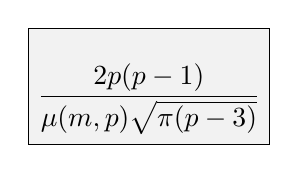
\begin{tikzpicture}
        		\node[draw,fill=black!5!,text height=0.84cm] (label) {$\dfrac{2p(p-1)}{\mu(m,p)\sqrt{\pi(p-3)}}$};
                \end{tikzpicture}\\ [1ex]
                where \hspace{0.2cm} $\mu(m,p) = \dfrac{1}{\sqrt{p-3}}\Phi^{-1}\left(1 - \dfrac{1}{m(p-1)}\right)$
             \end{tabular}} & 
            {\begin{tabular}{c}
                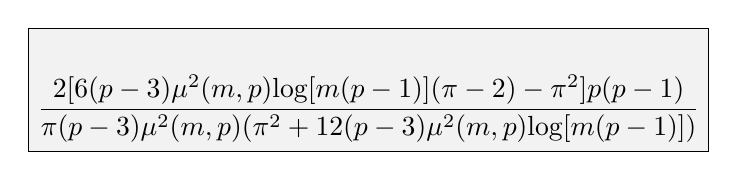
\begin{tikzpicture}
        	    \node[draw,fill=black!5!,text height=1cm] (label) {$\dfrac{2[6(p-3)\mu^2(m,p)\text{log}[m(p-1)](\pi-2) - \pi^2]p(p-1)}{\pi(p-3)\mu^2(m,p)(\pi^2+12(p-3)\mu^2(m,p)\text{log}[m(p-1)])}$};
                \end{tikzpicture} \\ [1ex]
               where \hspace{0.2cm} $\mu(m,p) = \dfrac{1}{\sqrt{p-3}}\Phi^{-1}\left(1 - \dfrac{1}{m(p-1)}\right)$
             \end{tabular}} & \\ [15ex] \hline
        & & & \\ [-2.4ex]
        {\begin{tabular}{c}$\text{GWAS}$ \\ [0.2ex] ($\textbf{d}_{\textbf{GM}}$) \end{tabular}} & 
        {\begin{tabular}{c}
                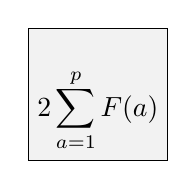
\begin{tikzpicture}
                \node[draw,fill=black!5!,text height=1cm] (label) {$2\dsum_{a=1}^{p}F(a)$};
                \end{tikzpicture} \\ [1ex]
                {\begin{tabular}{l} 
                where \\ [1ex]
        	    $F(a) = \left[2(1 - f_a)^3 f_a + 2f^3_a (1 - f_a) + (1 - f_a)^2 f^2_a\right]$, \\ [1ex]
        	    and $f_a$ is the probability of a minor allele at locus $a$.
        	    \end{tabular}}
       \end{tabular}}&         
       {\begin{tabular}{c}
                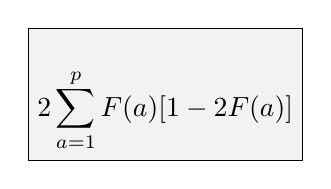
\begin{tikzpicture}
        	    \node[draw,fill=black!5!,text height=1cm] (label) {$2 \dsum_{a=1}^{p}F(a)[1 - 2F(a)]$};
                \end{tikzpicture} \\ [1ex]
                {\begin{tabular}{l}
        	    where \\ [1ex]
        	    $F(a) = \left[2(1 - f_a)^3 f_a + 2f^3_a (1 - f_a) + (1 - f_a)^2 f^2_a\right]$, \\ [1ex]
                and $f_a$ is the probability of a minor allele at locus $a$.
        	    \end{tabular}}
       \end{tabular}} & \\ [20ex] \hline
       {\begin{tabular}{c}$\text{GWAS}$ \\ [0.2ex] ($\textbf{d}_{\textbf{AM}}$) \end{tabular}} & 
       {\begin{tabular}{c}  
                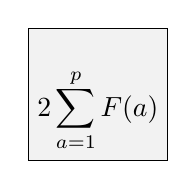
\begin{tikzpicture}
        		\node[draw,fill=black!5!,text height=1cm] (label) {$2\dsum_{a=1}^{p}F(a)$};
                \end{tikzpicture} \\ [1ex]
                {\begin{tabular}{l}
        		where \\ [1ex]
                $F(a) = \left[(1 - f_a)^3 f_a + f^3_a (1 - f_a) + (1 - f_a)^2 f^2_a\right]$, \\ [1ex]
                and $f_a$ is the probability of a minor allele at locus $a$.
                \end{tabular}}
       \end{tabular}}          & 
       {\begin{tabular}{c}
                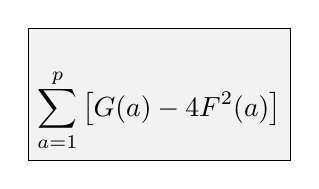
\begin{tikzpicture}
                \node[draw,fill=black!5!,text height=1cm] (label) {$\dsum_{a=1}^{p}\left[G(a) - 4F^2(a)\right]$};
                \end{tikzpicture} \\ [1ex]
                {\begin{tabular}{l}
                where \\ [1ex]
                $F(a) = \left[(1 - f_a)^3 f_a + f^3_a (1 - f_a) + f^3_a (1 - f_a) + (1 - f_a)^2 f^2_a\right]$, \\ [2ex]
                $G(a) = \left[(1 - f_a)^3 f_a + f^3_a (1 - f_a) + 2(1 - f_a)^2 f^2_a\right]$, \\ [1ex] 
                and $f_a$ is the probability of a minor allele at locus $a$.
                \end{tabular}}
       \end{tabular}} & \\ [25.7ex] \hline
        & & & \\ [-2ex]
       {\begin{tabular}{c} $\text{GWAS}$ \\ [0.2ex] ($\textbf{d}_{\textbf{TiTv}}$) \end{tabular}} &
       {\begin{tabular}{c}
               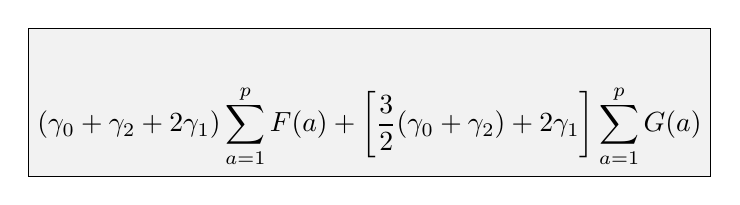
\begin{tikzpicture}
        	   \node[draw,fill=black!5!,text height=1.2cm] (label) {$(\gamma_0 + \gamma_2 + 2\gamma_1)\dsum_{a=1}^{p} F(a) + \left[\frac{3}{2}(\gamma_0+\gamma_2) + 2\gamma_1\right]\dsum_{a=1}^{p} G(a)$};
               \end{tikzpicture} \\ [1ex]
               {\begin{tabular}{l}
        	   where \\ [1ex]
        	   $F(a)=\left[(1-f_a)^3 f_a + f^3_a(1 - f_a)\right]$ and $G(a)=(1 - f_a)^2f^2_a$, \\ [1ex]
        	   $f_a$ is the probability of a minor allele at locus $a$, and $\gamma_0$, $\gamma_1$, \\ [1ex]
        	   and $\gamma_2$ are probabilities of PuPu, PuPy, and PyPy, \\ [1ex]
        	   respectively, at locus $a$.
        	   \end{tabular}}
       \end{tabular}}& 
      {\begin{tabular}{c}
               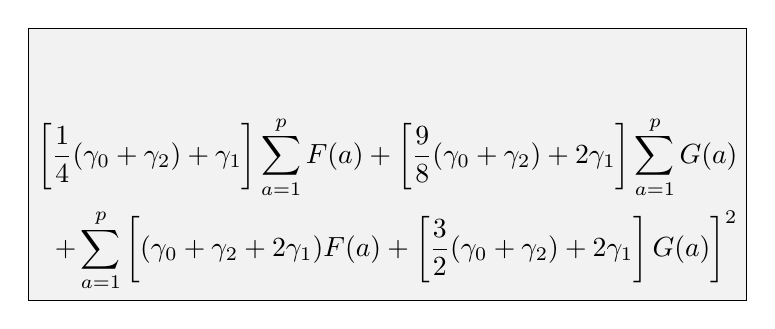
\begin{tikzpicture}
               \node[draw,fill=black!5!,text height=2.2cm] (label) {
                     $\begin{aligned}
                     \left[\frac{1}{4}(\gamma_0+\gamma_2)+\gamma_1\right]\dsum_{a=1}^{p}F(a) + \left[\frac{9}{8}(\gamma_0+\gamma_2)+2\gamma_1\right]\dsum_{a=1}^{p}G(a) \\
                     + \dsum_{a=1}^{p}\left[(\gamma_0+\gamma_2+2\gamma_1)F(a) + \left[\frac{3}{2}(\gamma_0+\gamma_2) + 2\gamma_1\right]G(a)\right]^2
                     \end{aligned}$
               };
               \end{tikzpicture} \\ [1ex]
            {\begin{tabular}{l}
            where \\ [1ex]
            $F(a)=\left[(1-f_a)^3 f_a + f^3_a(1 - f_a)\right]$ and $G(a)=(1 - f_a)^2f^2_a$, \\ [1ex]
            $f_a$ is the probability of a minor allele at locus $a$, and $\gamma_0$, $\gamma_1$, \\ [1ex]
            and $\gamma_2$ are probabilities of PuPu, PuPy, and PyPy, \\ [1ex]
            respectively, at locus $a$.
            \end{tabular}}
      \end{tabular}}       & \\ [35ex] \hline
		\end{tabular}
	\end{adjustbox}
	\end{table}
\end{center}

\end{document}